\chapter{Ergebnisse}

\section{Klassifizierung zwischen Tumor und no Tumor}

\subsection{Hyperparameter}

\begin{figure}[htbp]
  \centering
  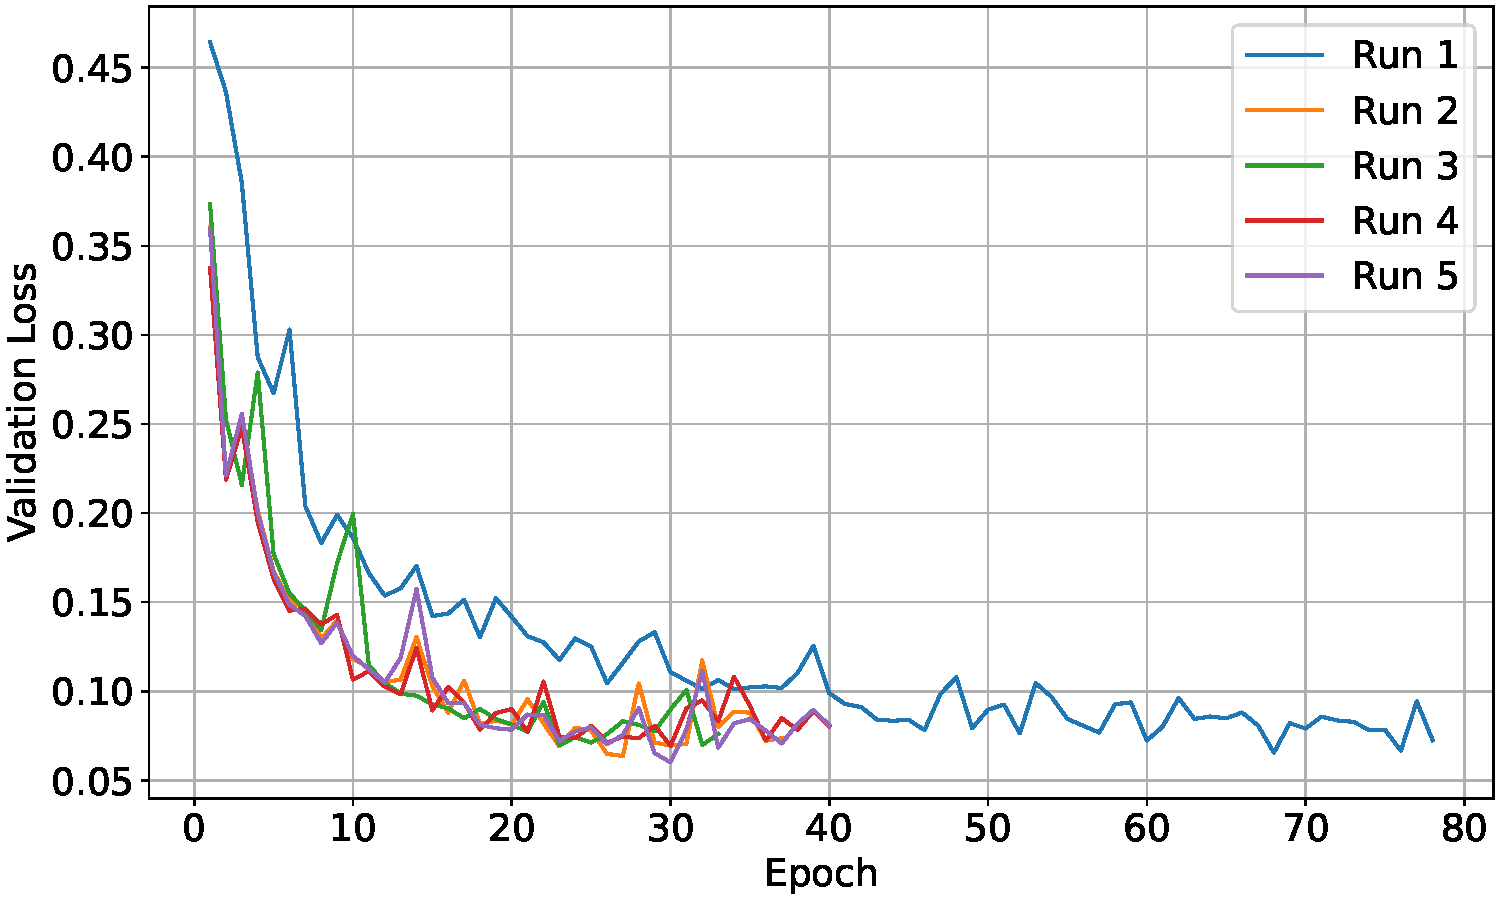
\includegraphics[scale=0.4]{plots/Val_loss_noTu_Tu.pdf}
  \caption{Darstellung des Validierungs Loss bei der Verwendung verschiedener Hyperparameter.}
  \label{fig:val_loss notu-tu}
\end{figure}

\begin{table}[htbp]
    \centering
    \resizebox{\textwidth}{!}{%
        \begin{tabular}{cccccccc}
            \toprule
            Runs & Batch Größe & Lernrate & Dropout & Validation Loss & Accuracy/$\%$ & Sensitivity & Specificity \\
            \midrule
            1 & 128 &0.005  & 0.55 & 0.072539 & 97.53231 & 0.97967 & 0.96774 \\
            2 & 128 &0.0005 & 0.5  & 0.073672 & 98.00235 & 0.98706 & 0.96774 \\
            3 & 16  &0.0001 & 0.5  & 0.076007 & 97.88484 & 0.97597 & 0.98387 \\
            4 & 128 &0.0005 & 0.4  & 0.080399 & 97.76733 & 0.97782 & 0.97742 \\
            5 & 128 &0.0005 & 0.5  & 0.080853 & 97.64982 & 0.98706 & 0.95806 \\
            \bottomrule
        \end{tabular}
    }
  \caption{.}
  \label{tab:hyperp notu-tu }
\end{table}

\subsection{Reduzierung der Trainingssamples}
\subsection{Augmentation}
\subsection{Reduzierung der Tumorsamples}

\section{Klassifizierung zwischen Glioma und Meningioma}

\subsection{Hyperparameter}
\begin{figure}[htbp]
  \centering
  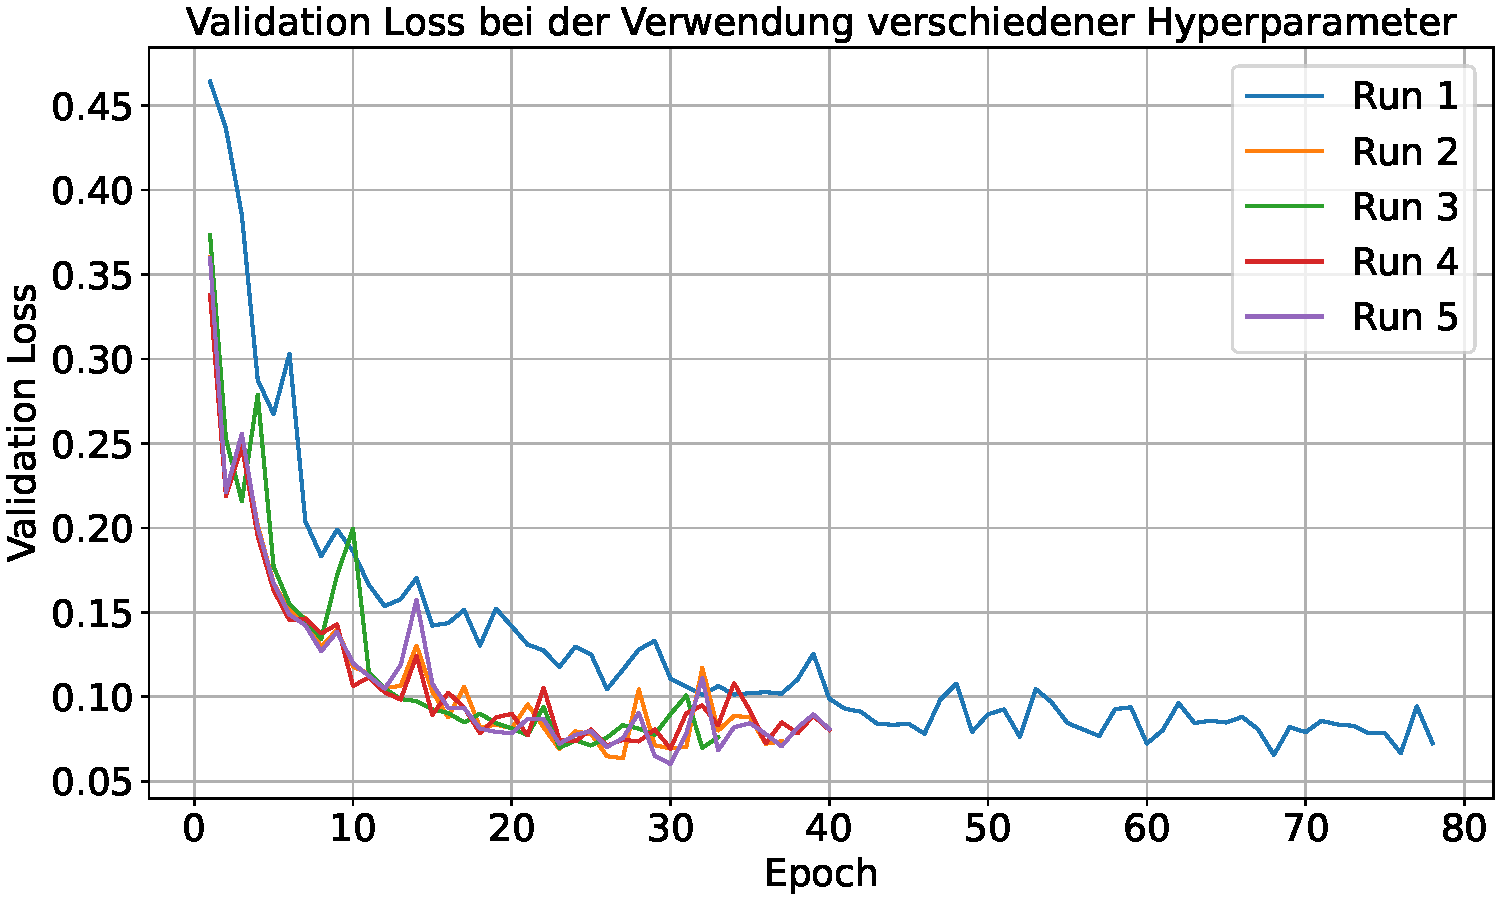
\includegraphics[scale=0.4]{plots/Val_loss_Gli_Men.pdf}
  \caption{Darstellung des Validierungs Loss bei der Verwendung verschiedener Hyperparameter.}
  \label{fig:val_loss gli-men}
\end{figure}

\begin{table}[htbp]
    \centering
    \resizebox{\textwidth}{!}{%
        \begin{tabular}{cccccccc}
            \toprule
            Runs & Batch Größe & Lernrate & Dropout & Validation Loss & Accuracy/$\%$ & Sensitivity & Specificity \\
            \midrule
            1 & 128 & 0.01  & 0.55 & 0.18943 & 92.29323 & 0.95402 & 0.89299 \\
            2 & 64  & 0.005 & 0.3  & 0.22499 & 93.23308 & 0.96935 & 0.89668 \\
            3 & 16  & 0.0005& 0.55 & 0.23146 & 93.98496 & 0.9272  & 0.95203 \\
            4 & 16  & 0.005 & 0.5  & 0.23453 & 92.66917 & 0.95402 & 0.90037 \\
            5 & 16  & 0.0005& 0.5  & 0.23829 & 93.42105 & 0.94253 & 0.9262 \\
            \bottomrule
        \end{tabular}
    }
  \caption{.}
  \label{tab:hyperp notu-tu }
\end{table}

\subsection{Reduzierung der Trainingssamples}
\subsection{Augmentation}
\subsection{Reduzierung der Gliomasamples}

